% Options for packages loaded elsewhere
\PassOptionsToPackage{unicode}{hyperref}
\PassOptionsToPackage{hyphens}{url}
\documentclass[
  ignorenonframetext,
]{beamer}
\newif\ifbibliography
\usepackage{pgfpages}
\setbeamertemplate{caption}[numbered]
\setbeamertemplate{caption label separator}{: }
\setbeamercolor{caption name}{fg=normal text.fg}
\beamertemplatenavigationsymbolsempty
% remove section numbering
\setbeamertemplate{part page}{
  \centering
  \begin{beamercolorbox}[sep=16pt,center]{part title}
    \usebeamerfont{part title}\insertpart\par
  \end{beamercolorbox}
}
\setbeamertemplate{section page}{
  \centering
  \begin{beamercolorbox}[sep=12pt,center]{section title}
    \usebeamerfont{section title}\insertsection\par
  \end{beamercolorbox}
}
\setbeamertemplate{subsection page}{
  \centering
  \begin{beamercolorbox}[sep=8pt,center]{subsection title}
    \usebeamerfont{subsection title}\insertsubsection\par
  \end{beamercolorbox}
}
% Prevent slide breaks in the middle of a paragraph
\widowpenalties 1 10000
\raggedbottom
\AtBeginPart{
  \frame{\partpage}
}
\AtBeginSection{
  \ifbibliography
  \else
    \frame{\sectionpage}
  \fi
}
\AtBeginSubsection{
  \frame{\subsectionpage}
}
\usepackage{iftex}
\ifPDFTeX
  \usepackage[T1]{fontenc}
  \usepackage[utf8]{inputenc}
  \usepackage{textcomp} % provide euro and other symbols
\else % if luatex or xetex
  \usepackage{unicode-math} % this also loads fontspec
  \defaultfontfeatures{Scale=MatchLowercase}
  \defaultfontfeatures[\rmfamily]{Ligatures=TeX,Scale=1}
\fi
\usepackage{lmodern}
\ifPDFTeX\else
  % xetex/luatex font selection
\fi
% Use upquote if available, for straight quotes in verbatim environments
\IfFileExists{upquote.sty}{\usepackage{upquote}}{}
\IfFileExists{microtype.sty}{% use microtype if available
  \usepackage[]{microtype}
  \UseMicrotypeSet[protrusion]{basicmath} % disable protrusion for tt fonts
}{}
\makeatletter
\@ifundefined{KOMAClassName}{% if non-KOMA class
  \IfFileExists{parskip.sty}{%
    \usepackage{parskip}
  }{% else
    \setlength{\parindent}{0pt}
    \setlength{\parskip}{6pt plus 2pt minus 1pt}}
}{% if KOMA class
  \KOMAoptions{parskip=half}}
\makeatother
\usepackage{color}
\usepackage{fancyvrb}
\newcommand{\VerbBar}{|}
\newcommand{\VERB}{\Verb[commandchars=\\\{\}]}
\DefineVerbatimEnvironment{Highlighting}{Verbatim}{commandchars=\\\{\}}
% Add ',fontsize=\small' for more characters per line
\newenvironment{Shaded}{}{}
\newcommand{\AlertTok}[1]{\textcolor[rgb]{1.00,0.00,0.00}{\textbf{#1}}}
\newcommand{\AnnotationTok}[1]{\textcolor[rgb]{0.38,0.63,0.69}{\textbf{\textit{#1}}}}
\newcommand{\AttributeTok}[1]{\textcolor[rgb]{0.49,0.56,0.16}{#1}}
\newcommand{\BaseNTok}[1]{\textcolor[rgb]{0.25,0.63,0.44}{#1}}
\newcommand{\BuiltInTok}[1]{\textcolor[rgb]{0.00,0.50,0.00}{#1}}
\newcommand{\CharTok}[1]{\textcolor[rgb]{0.25,0.44,0.63}{#1}}
\newcommand{\CommentTok}[1]{\textcolor[rgb]{0.38,0.63,0.69}{\textit{#1}}}
\newcommand{\CommentVarTok}[1]{\textcolor[rgb]{0.38,0.63,0.69}{\textbf{\textit{#1}}}}
\newcommand{\ConstantTok}[1]{\textcolor[rgb]{0.53,0.00,0.00}{#1}}
\newcommand{\ControlFlowTok}[1]{\textcolor[rgb]{0.00,0.44,0.13}{\textbf{#1}}}
\newcommand{\DataTypeTok}[1]{\textcolor[rgb]{0.56,0.13,0.00}{#1}}
\newcommand{\DecValTok}[1]{\textcolor[rgb]{0.25,0.63,0.44}{#1}}
\newcommand{\DocumentationTok}[1]{\textcolor[rgb]{0.73,0.13,0.13}{\textit{#1}}}
\newcommand{\ErrorTok}[1]{\textcolor[rgb]{1.00,0.00,0.00}{\textbf{#1}}}
\newcommand{\ExtensionTok}[1]{#1}
\newcommand{\FloatTok}[1]{\textcolor[rgb]{0.25,0.63,0.44}{#1}}
\newcommand{\FunctionTok}[1]{\textcolor[rgb]{0.02,0.16,0.49}{#1}}
\newcommand{\ImportTok}[1]{\textcolor[rgb]{0.00,0.50,0.00}{\textbf{#1}}}
\newcommand{\InformationTok}[1]{\textcolor[rgb]{0.38,0.63,0.69}{\textbf{\textit{#1}}}}
\newcommand{\KeywordTok}[1]{\textcolor[rgb]{0.00,0.44,0.13}{\textbf{#1}}}
\newcommand{\NormalTok}[1]{#1}
\newcommand{\OperatorTok}[1]{\textcolor[rgb]{0.40,0.40,0.40}{#1}}
\newcommand{\OtherTok}[1]{\textcolor[rgb]{0.00,0.44,0.13}{#1}}
\newcommand{\PreprocessorTok}[1]{\textcolor[rgb]{0.74,0.48,0.00}{#1}}
\newcommand{\RegionMarkerTok}[1]{#1}
\newcommand{\SpecialCharTok}[1]{\textcolor[rgb]{0.25,0.44,0.63}{#1}}
\newcommand{\SpecialStringTok}[1]{\textcolor[rgb]{0.73,0.40,0.53}{#1}}
\newcommand{\StringTok}[1]{\textcolor[rgb]{0.25,0.44,0.63}{#1}}
\newcommand{\VariableTok}[1]{\textcolor[rgb]{0.10,0.09,0.49}{#1}}
\newcommand{\VerbatimStringTok}[1]{\textcolor[rgb]{0.25,0.44,0.63}{#1}}
\newcommand{\WarningTok}[1]{\textcolor[rgb]{0.38,0.63,0.69}{\textbf{\textit{#1}}}}
\usepackage{longtable,booktabs,array}
\newcounter{none} % for unnumbered tables
\usepackage{calc} % for calculating minipage widths
\usepackage{caption}
% Make caption package work with longtable
\makeatletter
\def\fnum@table{\tablename~\thetable}
\makeatother
\usepackage{graphicx}
\makeatletter
\newsavebox\pandoc@box
\newcommand*\pandocbounded[1]{% scales image to fit in text height/width
  \sbox\pandoc@box{#1}%
  \Gscale@div\@tempa{\textheight}{\dimexpr\ht\pandoc@box+\dp\pandoc@box\relax}%
  \Gscale@div\@tempb{\linewidth}{\wd\pandoc@box}%
  \ifdim\@tempb\p@<\@tempa\p@\let\@tempa\@tempb\fi% select the smaller of both
  \ifdim\@tempa\p@<\p@\scalebox{\@tempa}{\usebox\pandoc@box}%
  \else\usebox{\pandoc@box}%
  \fi%
}
% Set default figure placement to htbp
\def\fps@figure{htbp}
\makeatother
\setlength{\emergencystretch}{3em} % prevent overfull lines
\providecommand{\tightlist}{%
  \setlength{\itemsep}{0pt}\setlength{\parskip}{0pt}}
% Slide layout defaults for warning-clean scientific decks.
\usepackage{etoolbox}
\IfFileExists{xurl.sty}{\usepackage{xurl}}{}
\IfFileExists{seqsplit.sty}{\usepackage{seqsplit}}{\newcommand{\seqsplit}[1]{#1}}
\protected\def\breakseq#1{\seqsplit{#1}}
\protected\def\breaktt#1{\begingroup\ttfamily\seqsplit{#1}\endgroup}
\setlength{\emergencystretch}{6em}
\tolerance=5000
\hbadness=10000
\hfuzz=1pt
\setlength{\tabcolsep}{2pt}
\AtBeginEnvironment{longtable}{\tiny\renewcommand{\arraystretch}{0.86}\setlength{\tabcolsep}{1pt}}
\AtBeginEnvironment{tabular}{\tiny\renewcommand{\arraystretch}{0.86}\setlength{\tabcolsep}{1pt}}

% Natbib and cross-reference fallbacks — slides don't load natbib
% or cleveref, but combined-PDF manuscript prose may emit these
% commands. The fallback renders citations as a bracketed key list
% and cross-references as detokenized labels so slides don't fail on
% undefined control sequences or raw underscores. \providecommand is
% a no-op if packages load later.
\providecommand{\citep}[1]{[#1]}
\providecommand{\citet}[1]{#1}
\providecommand{\citealp}[1]{#1}
\providecommand{\citeauthor}[1]{#1}
\providecommand{\citeyear}[1]{#1}
\providecommand{\cref}[1]{\texttt{\detokenize{#1}}}
\providecommand{\Cref}[1]{\texttt{\detokenize{#1}}}

\newtheorem{proposition}{Proposition}
\newtheorem{hypothesis}{Hypothesis}
\usepackage{bookmark}
\IfFileExists{xurl.sty}{\usepackage{xurl}}{} % add URL line breaks if available
\urlstyle{same}
% fallback for those not using the hyperref driver hyperxmp:
\makeatletter
\@ifundefined{xmpquote}{\newcommand{\xmpquote}[1]{#1}}{}
\makeatother
\hypersetup{
  hidelinks,
  pdfcreator={LaTeX via pandoc}}

\author{\texorpdfstring{}{}}
\date{}

\begin{document}

\section{Tools: Executable Entry Points}\label{sec:tools}

\begin{frame}[fragile,allowframebreaks]{What Is a Tool?}
\protect\phantomsection\label{what-is-a-tool}
A \textbf{tool} in the template repository is a directory under
\texttt{tools/\textless{}scope\textgreater{}/\textless{}name\textgreater{}/}
that packages one or more executable scripts behind a typed manifest
(\texttt{tools.yaml}). Tools provide the third layer of the resource
architecture: where fonds supply static data and rules supply governance
constraints, tools supply \emph{behaviour} --- computations, validation
runs, and agent skill invocations that projects can trigger without
re-implementing the underlying logic.

The tools layer deliberately mirrors the Unix philosophy of small,
composable utilities that communicate through standard interfaces
\breakseq{[@Raymond2003art]}. Each tool declares its entrypoints (shell
scripts), its invocation contract (stdin/stdout/exit-code semantics),
and its capabilities (type, version, tags) in a single manifest file.
Consumers invoke tools through the \texttt{tools\_invoker} module
without needing to understand the tool's implementation details --- a
textbook application of the Facade pattern \breakseq{[@Gamma1994design]}.
\end{frame}

\begin{frame}[fragile,allowframebreaks]{The \texttt{tools.yaml}
Manifest}
\protect\phantomsection\label{the-tools.yaml-manifest}
Every tool root must contain a \texttt{tools.yaml} manifest with the
following fields:

\begin{Shaded}
\begin{Highlighting}[]
\FunctionTok{type}\KeywordTok{:}\AttributeTok{ code\_executor | validator | skill | agent | renderer}
\FunctionTok{description}\KeywordTok{:}\AttributeTok{ }\StringTok{"Human{-}readable description of the tool"}
\FunctionTok{version}\KeywordTok{:}\AttributeTok{ }\StringTok{"1.0.0"}
\FunctionTok{tags}\KeywordTok{:}\AttributeTok{ }\KeywordTok{[}\AttributeTok{curated}\KeywordTok{,}\AttributeTok{ exemplar}\KeywordTok{,}\AttributeTok{ production}\KeywordTok{,}\AttributeTok{ experimental}\KeywordTok{]}
\FunctionTok{creator}\KeywordTok{:}\AttributeTok{ }\StringTok{"org/repo"}
\FunctionTok{license}\KeywordTok{:}\AttributeTok{ }\StringTok{"Apache{-}2.0"}
\FunctionTok{entrypoints}\KeywordTok{:}
\AttributeTok{  }\KeywordTok{{-}}\AttributeTok{ scripts/run.sh}
\AttributeTok{  }\KeywordTok{{-}}\AttributeTok{ scripts/validate.sh}
\end{Highlighting}
\end{Shaded}

The \texttt{type} field determines the invocation contract the consumer
should expect. The \texttt{entrypoints} list names the scripts that must
exist on disk; the \texttt{tools\_invoker} module validates their
presence at discovery time rather than at invocation time, making
failures visible early in the pipeline rather than at runtime.
@fig:toolcontract visualises the stdin/stdout/exit-code contract for all
three template tools side by side; note that the \emph{shape} of stdin
and stdout differs per tool while the \emph{presence} of a well-defined
contract does not --- this is what makes \texttt{tools\_invoker} able to
discover and validate any tool generically without knowing its payload
schema.

\begin{figure}
\centering
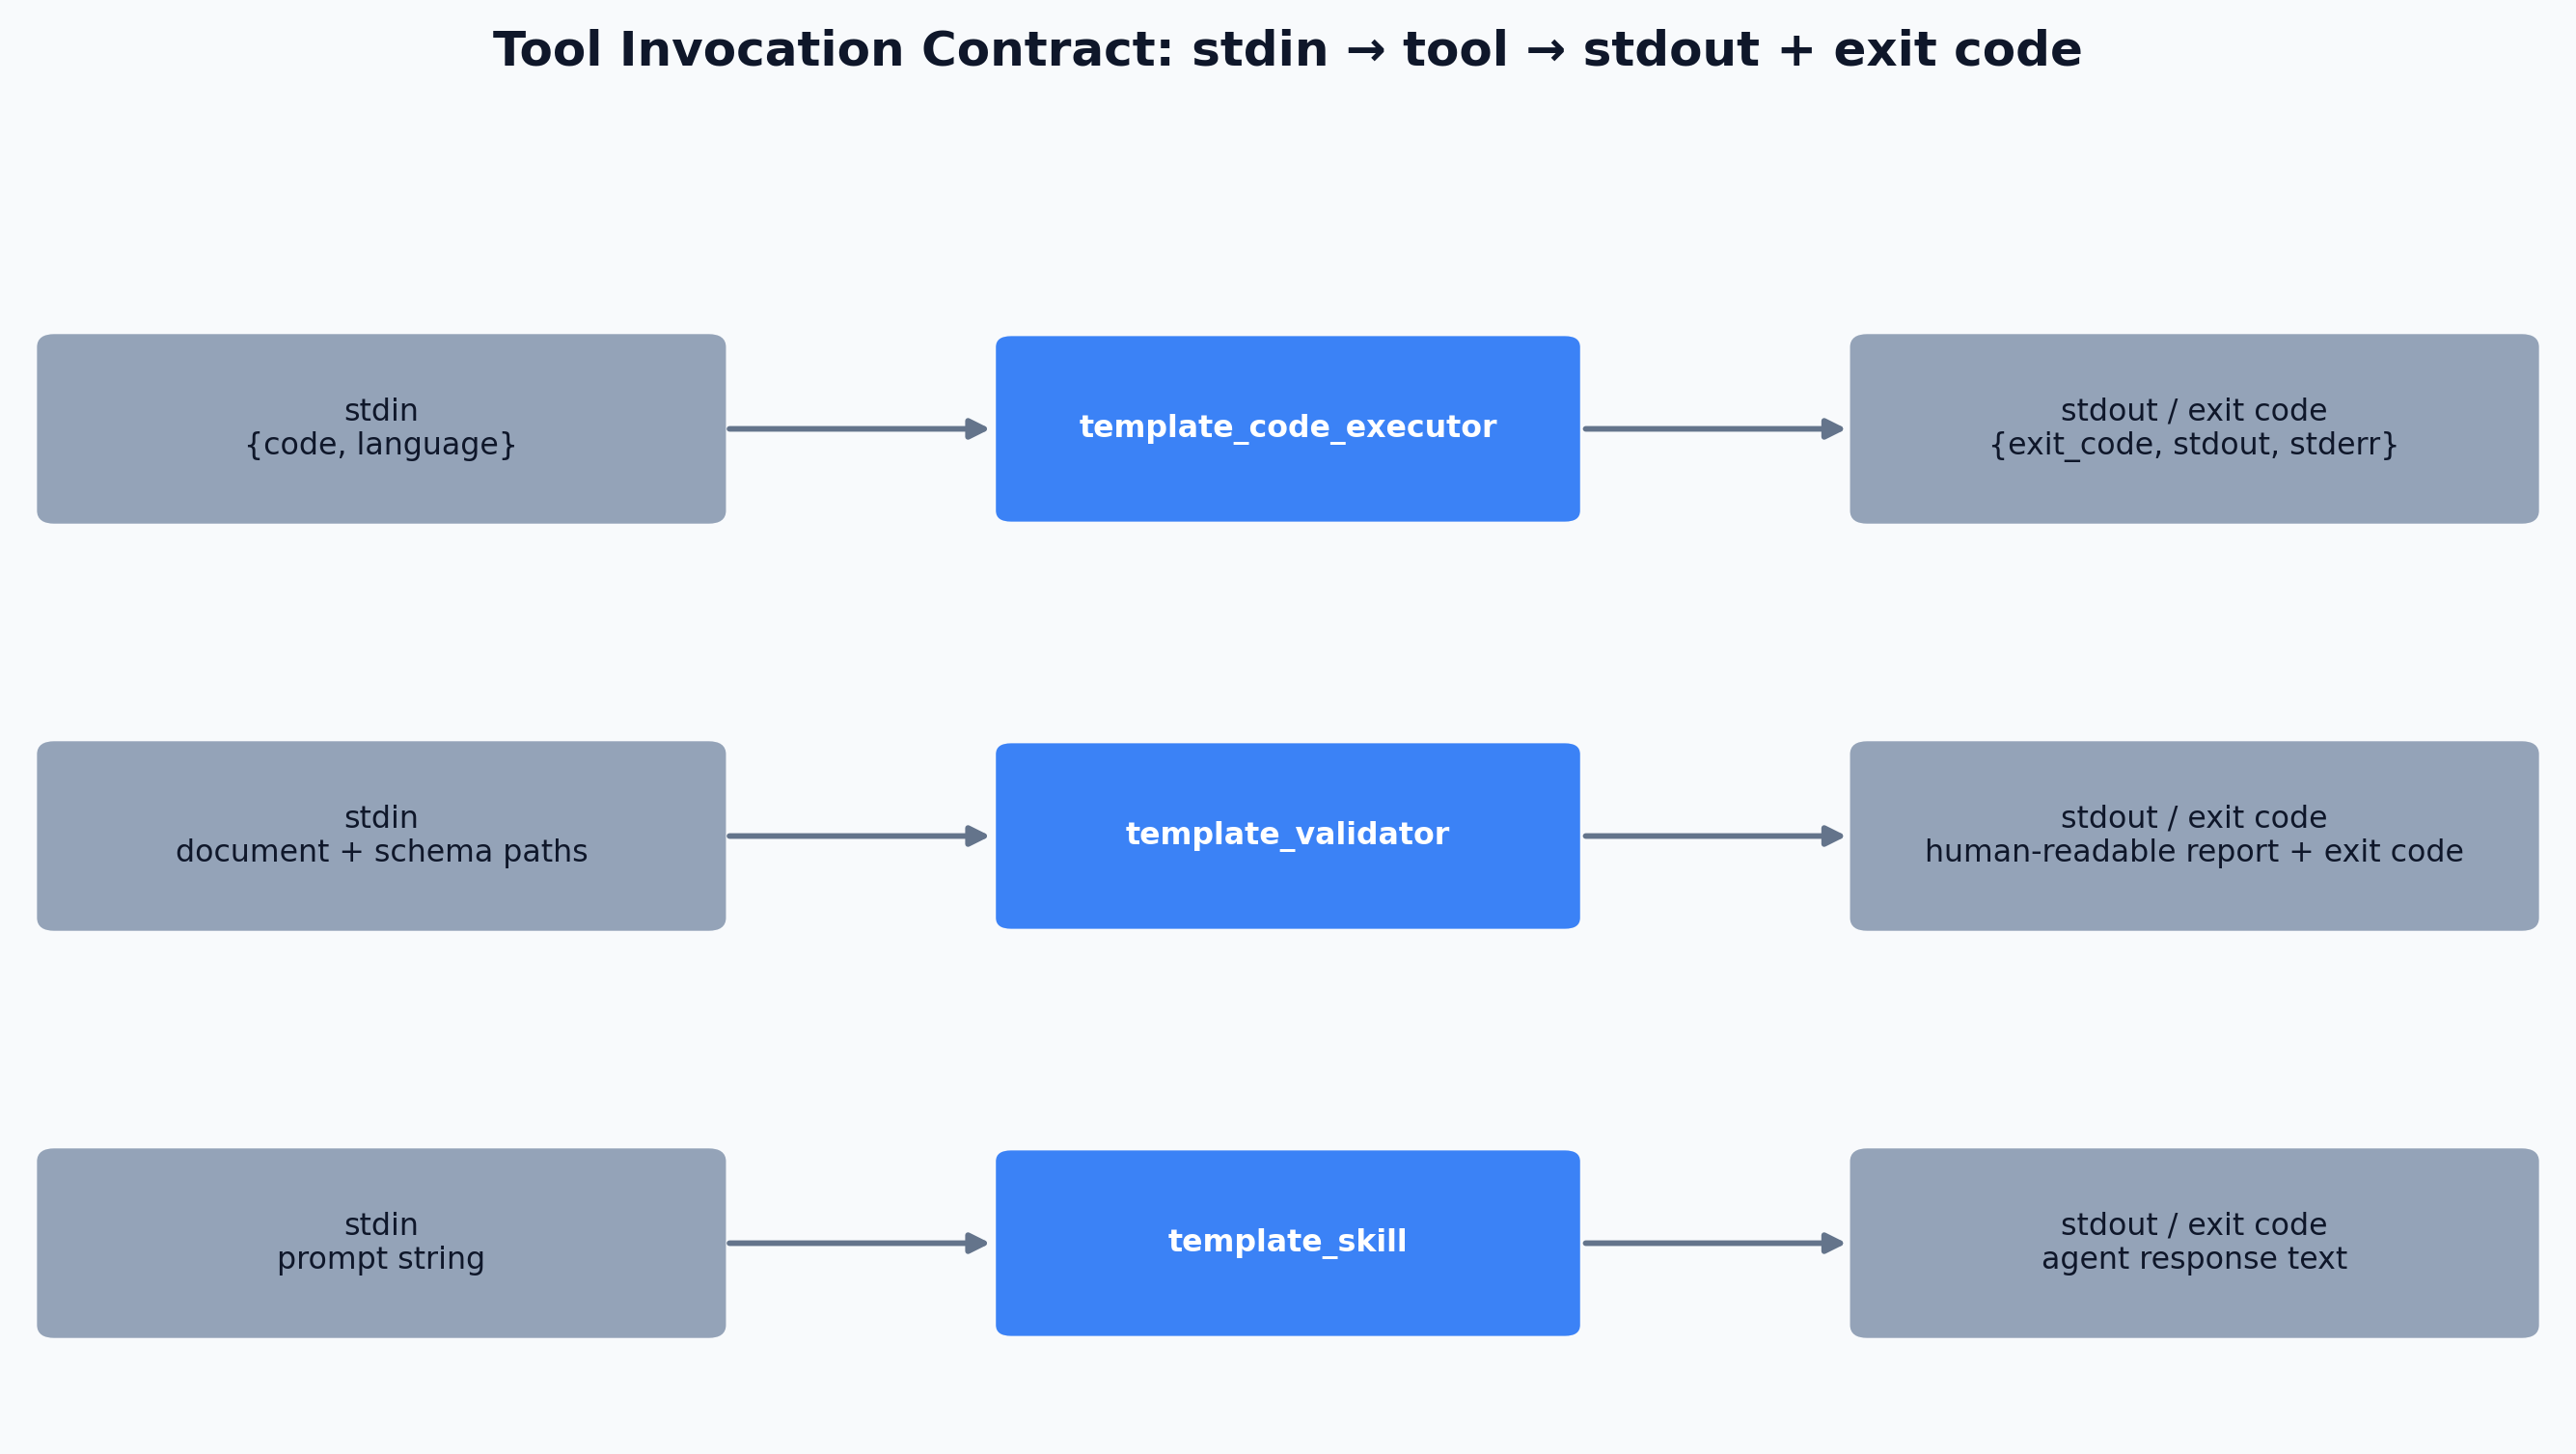
\includegraphics[width=0.9\linewidth,height=0.46\textheight,keepaspectratio,alt={Invocation contract for the three template tools: stdin payload, tool behaviour, and stdout/exit-code shape.}]{../figures/tool_contract.png}
\caption{Invocation contract for the three template tools: stdin
payload, tool behaviour, and stdout/exit-code
shape.}\label{fig:toolcontract}
\end{figure}
\end{frame}

\begin{frame}[fragile,allowframebreaks]{The Three Template Tools}
\protect\phantomsection\label{the-three-template-tools}
\begin{block}{\breaktt{template\_code\_executor}}
\protect\phantomsection\label{template_code_executor}
A generic code execution tool that accepts a JSON payload on standard
input and returns execution results as JSON. The invocation contract is:

{\def\LTcaptype{none} % do not increment counter
\begin{longtable}[]{@{}
  >{\raggedright\arraybackslash}p{(\linewidth - 6\tabcolsep) * \real{0.2500}}
  >{\raggedright\arraybackslash}p{(\linewidth - 6\tabcolsep) * \real{0.2500}}
  >{\raggedright\arraybackslash}p{(\linewidth - 6\tabcolsep) * \real{0.2500}}
  >{\raggedright\arraybackslash}p{(\linewidth - 6\tabcolsep) * \real{0.2500}}@{}}
\toprule\noalign{}
\begin{minipage}[b]{\linewidth}\raggedright
Entrypoint
\end{minipage} & \begin{minipage}[b]{\linewidth}\raggedright
stdin
\end{minipage} & \begin{minipage}[b]{\linewidth}\raggedright
stdout
\end{minipage} & \begin{minipage}[b]{\linewidth}\raggedright
exit code
\end{minipage} \\
\midrule\noalign{}
\endhead
\texttt{scripts/run.sh} & \texttt{\{"code":\ str,\ "language":\ str\}} &
\texttt{\{"exit\_code":\ int,\ "stdout":\ str,\ "stderr":\ str\}} & 0 =
success \\
\breaktt{scripts/validate.sh} & --- & Human-readable validation report &
0 = valid \\
\bottomrule\noalign{}
\end{longtable}
}

The code executor exemplifies tools that wrap a computational
capability. The JSON-in/JSON-out contract makes it easily composable
with pipeline orchestrators and agent frameworks.
\end{block}

\begin{block}{\breaktt{template\_validator}}
\protect\phantomsection\label{template_validator}
A JSON Schema validation tool. It reads a target document and a schema
from disk and reports validation results in human-readable form. The
entrypoint \breaktt{scripts/validate.sh} exits 0 when the document is
valid and non-zero with a detailed error message otherwise. The
validator tool is used in the project pipeline to validate
\breaktt{manuscript\_variables.json} against its expected schema before
manuscript rendering.
\end{block}

\begin{block}{\texttt{template\_skill}}
\protect\phantomsection\label{template_skill}
An agent skill invocation tool that wraps a Hermes-compatible skill
definition. The entrypoint \breaktt{scripts/invoke.sh} accepts a prompt
string on standard input and returns the agent response as text. This
tool type bridges the repository's tool architecture with external agent
frameworks, demonstrating that the same manifest-and-entrypoint pattern
applies equally to computational tools and AI agents.

Unlike the two tools above, \breaktt{scripts/invoke.sh} requires a real
\texttt{OPENAI\_API\_KEY} and makes a paid network call to
\texttt{api.openai.com} --- it is therefore never invoked by this
project's tests or pipeline, by design. Offline reproducibility is a
stated requirement of this exemplar (see the front-matter
Reproducibility Checklist), and no CI job in this repository injects
\texttt{OPENAI\_API\_KEY} into this project's test run.
\breaktt{template\_code\_executor} and \breaktt{template\_validator}, by
contrast, are fully local and deterministic --- see the Execution-Proof
Testing subsection below for how this project actually exercises them.
\end{block}
\end{frame}

\begin{frame}[fragile,allowframebreaks]{The \texttt{tools\_invoker}
Module}
\protect\phantomsection\label{the-tools_invoker-module}
The \breaktt{src/tools\_invoker.py} module provides three public
functions:

\begin{Shaded}
\begin{Highlighting}[]
\ImportTok{from}\NormalTok{ src.tools\_invoker }\ImportTok{import}\NormalTok{ (}
\NormalTok{    discover\_tools,}
\NormalTok{    get\_tool\_entrypoints,}
\NormalTok{    validate\_tool\_scripts\_exist,}
\NormalTok{)}

\NormalTok{tools }\OperatorTok{=}\NormalTok{ discover\_tools()}
\CommentTok{\# → [\{"name": "template\_code\_executor", "manifest": \{...\}\}, ...]}

\NormalTok{eps }\OperatorTok{=}\NormalTok{ get\_tool\_entrypoints(}\StringTok{"template\_code\_executor"}\NormalTok{)}
\CommentTok{\# → ["scripts/run.sh", "scripts/validate.sh"]}

\NormalTok{result }\OperatorTok{=}\NormalTok{ validate\_tool\_scripts\_exist(}\StringTok{"template\_code\_executor"}\NormalTok{)}
\CommentTok{\# → \{"status": "ok" | "partial" | "missing", "missing\_scripts": [...]\}}
\end{Highlighting}
\end{Shaded}

\breaktt{discover\_tools()} scans \breaktt{tools/templates/} and returns
one \texttt{ToolEntry} per subdirectory, regardless of whether a
manifest is present: a directory with a parseable \texttt{tools.yaml}
gets \texttt{manifest=\{...\}}; a directory with no manifest, or one
that fails to parse, gets \texttt{manifest=None} plus a logged warning.
Discovery itself never raises and never drops a directory from the
result --- the \emph{interpretation} of ``not a real tool yet'' is left
to the caller (\breaktt{get\_tool\_entrypoints()} and
\breaktt{validate\_tool\_scripts\_exist()} both return an
empty/\texttt{"missing"} result for a \texttt{None} manifest), which
keeps discovery and validation as separate, independently testable
concerns.

\breaktt{validate\_tool\_scripts\_exist()} iterates over the manifest's
\texttt{entrypoints} list and checks each path against the filesystem.
It returns a structured result distinguishing between tools that are
fully ready (\texttt{"ok"}), partially configured (\texttt{"partial"}
--- some scripts missing), and entirely absent (\texttt{"missing"}). In
the current integration run, \textbf{3 tools} were discovered
(@fig:counts), all with valid manifests.
\end{frame}

\begin{frame}[fragile,allowframebreaks]{Tool Discovery and
Reproducibility}
\protect\phantomsection\label{tool-discovery-and-reproducibility}
The tools layer contributes to reproducibility by making the
\emph{availability} of computational capabilities explicit and
checkable. A project that hard-codes a path to a tool script becomes
brittle when the repository is reorganised. By contrast, a project that
calls \breaktt{discover\_tools()} and checks
\breaktt{validate\_tool\_scripts\_exist()} will detect missing
entrypoints at pipeline initialisation time and report them clearly,
rather than failing silently at execution time
\breakseq{[@Stodden2016enhancing]}. This shift from implicit to explicit
dependency declaration is a key design principle of the template
architecture (see @fig:architecture).
\end{frame}

\begin{frame}[fragile,allowframebreaks]{Tool Composition and Failure
Modes}
\protect\phantomsection\label{tool-composition-and-failure-modes}
Because every tool exposes the same discovery contract (manifest +
entrypoint list), tools compose without any consumer-side
special-casing. A pipeline stage that wants ``any validator'' can call
\breaktt{discover\_tools()}, filter the result list on
\texttt{manifest{[}"type"{]}\ ==\ "validator"}, and invoke whichever
\breaktt{template\_validator}-typed tool it finds --- without hard-coding
\breaktt{template\_validator} by name. This composability comes with
three failure modes that \texttt{tools\_invoker} handles explicitly
rather than leaving to the caller:

\begin{enumerate}
\tightlist
\item
  \textbf{Manifest present, entrypoint missing.}
  \breaktt{discover\_tools()} finds a parseable \texttt{tools.yaml}
  declaring \texttt{scripts/run.sh}, but the file does not exist.
  \breaktt{validate\_tool\_scripts\_exist()} surfaces this as
  \breaktt{status="partial"} with the specific missing path in
  \texttt{missing\_scripts}, catching the defect at discovery time
  instead of waiting for a caller to try executing the script.
\item
  \textbf{Manifest missing entirely.} A directory under
  \breaktt{tools/templates/} exists but has no \texttt{tools.yaml}.
  \breaktt{discover\_tools()} still returns a \texttt{ToolEntry} for it
  (with \texttt{manifest=None}, so the caller can see it exists), but
  \breaktt{get\_tool\_entrypoints()} and
  \breaktt{validate\_tool\_scripts\_exist()} both treat a \texttt{None}
  manifest as ``not yet a tool,'' returning an empty collection or
  \texttt{"missing"} status without ever raising --- this matters for
  partially-scaffolded work-in-progress tool directories created by a
  parallel agent.
\item
  \textbf{Manifest malformed YAML.} The same graceful-degradation
  pattern from @sec:pools applies here: a parse error is caught and
  logged, and the offending tool is quietly excluded from the discovery
  result, leaving the pipeline free to continue with everything else it
  found.
\end{enumerate}

Each of these is a distinct, testable branch in
\breaktt{tests/test\_tools\_invoker.py}, and each maps to one row of the
resilience taxonomy in @fig:resilience.
\end{frame}

\begin{frame}[fragile,allowframebreaks]{Execution-Proof Testing: Beyond
Manifest Checking}
\protect\phantomsection\label{execution-proof-testing-beyond-manifest-checking}
Everything described so far --- discovery, entrypoint-existence
validation, the three failure modes above --- is \emph{structural}: it
confirms a tool's files are present and well-formed without ever running
them. \breaktt{src/tools\_invoker.py}'s public API deliberately stays
that way, because subprocess execution is exactly the kind of operation
that can raise (a missing \texttt{bash}/\texttt{jq}/\texttt{python3}
binary, a permission error, a timeout), and this project's readers are
contracted to degrade gracefully rather than propagate exceptions (see
@sec:pools).

The test suite closes this gap without weakening that contract:
\breaktt{tests/test\_tools\_invoker.py} genuinely subprocess-invokes the
two fully local, deterministic tools and asserts on their real output,
rather than only checking that their scripts exist.

\begin{itemize}
\tightlist
\item
  \textbf{\breaktt{template\_code\_executor}}:
  \breaktt{TestInvokeCodeExecutor} pipes
  \texttt{\{"code":\ "print(2\ +\ 2)",\ "language":\ "python"\}} into
  the real \texttt{scripts/run.sh} and asserts the parsed JSON result
  has \breaktt{exit\_code\ ==\ 0} and \texttt{"4"} in \texttt{stdout} ---
  and, as a negative control, pipes code that calls
  \breaktt{raise\ SystemExit(3)} and asserts the real
  \breaktt{exit\_code\ ==\ 3} comes back.
\item
  \textbf{\breaktt{template\_validator}}: \breaktt{TestInvokeValidator}
  pipes a schema-conformant document into the real
  \breaktt{scripts/validate.sh} and asserts \breaktt{returncode\ ==\ 0}
  and \texttt{"VALID"} in stdout; a document missing the
  \texttt{version} field required by the tool's own \texttt{schema.json}
  is asserted to return \breaktt{returncode\ ==\ 1} and
  \texttt{"INVALID"} --- a genuine, schema-verified violation, not an
  assumed one.
\end{itemize}

Both test classes are guarded with \breaktt{pytest.mark.skipif} on the
real runtime dependency each script needs
(\texttt{timeout}/\texttt{gtimeout} plus \texttt{jq} for the code
executor; the \texttt{jsonschema} package for the validator), so a
missing binary skips the test cleanly instead of failing it --- on the
machine this manuscript was rendered on, the code-executor tests skip
(no \texttt{timeout}/\texttt{gtimeout} on this macOS host) while the
validator tests run for real, which is itself a demonstration of the
skip-guard working as intended rather than masking a failure.
\end{frame}

\end{document}
